
\documentclass{article}
\usepackage{pgfplots}
\usepackage{pgfplotstable}
\usepackage{tikz}
\pgfplotsset{compat=1.8}
\begin{document}
    \begin{figure*}[t]
        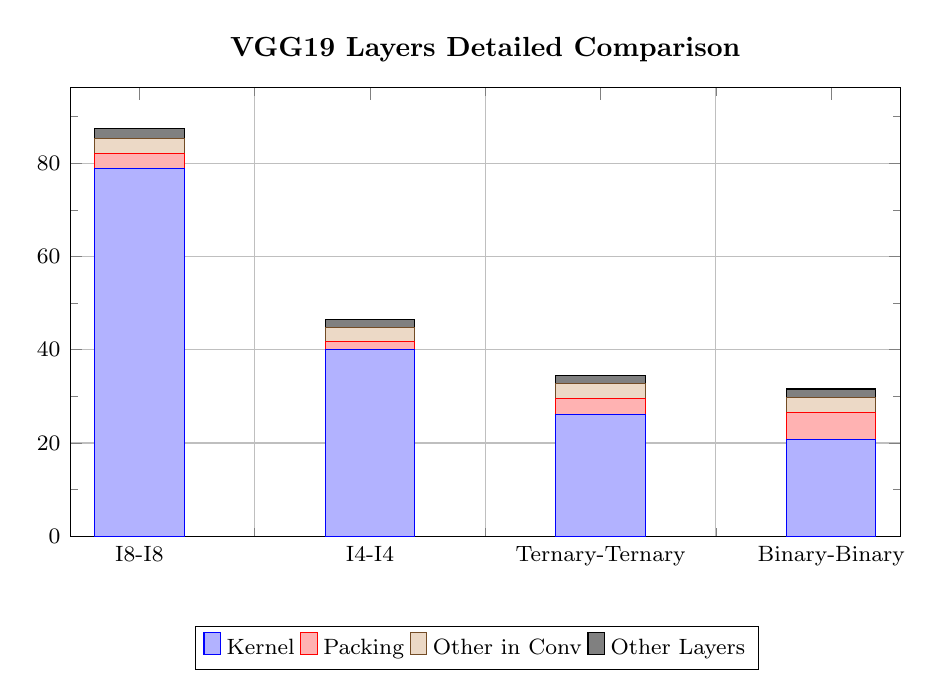
\begin{tikzpicture}
            \begin{axis}[
                ybar stacked,
                ymin=0.0,
                width=\linewidth,
                height=\axisdefaultheight,
                tick label style={font=\footnotesize},
                legend style={font=\tiny},
                label style={font=\footnotesize},
                symbolic x coords={I8-I8, I4-I4, Ternary-Ternary, Binary-Binary},
                xtick=data,
                % ytick={0.60,0.80,1.0,1.2,1.4,1.6,1.8,2.0,2.2,2.4,2.6,2.8,3.0},
                align={center},
                bar width=7.5ex,
                legend columns=7,
                legend style={at={(0.49,-0.2)},anchor=north,font=\footnotesize},
                title=\textbf{VGG19 Layers Detailed Comparison},
                ymajorgrids,
                xminorgrids = true,
                minor tick num=1
                ]
                \addplot coordinates { (I8-I8,78.88) (I4-I4,40.15) (Ternary-Ternary,26.02) (Binary-Binary,20.66) };
                \addplot coordinates { (I8-I8,3.28) (I4-I4,1.55) (Ternary-Ternary,3.58) (Binary-Binary,5.89) };
                \addplot coordinates { (I8-I8,3.25) (I4-I4,3.10) (Ternary-Ternary,3.21) (Binary-Binary,3.24) };
                \addplot coordinates { (I8-I8,2.03) (I4-I4,1.67) (Ternary-Ternary,1.63) (Binary-Binary,1.80) };
                \legend{
                    Kernel,
                    Packing,
                    Other in Conv,
                    Other Layers,
                };
            \end{axis}
        \end{tikzpicture}
    \end{figure*}
\end{document}
